\chapter{{\it Elib Joystick}} \label{app:joystick}
  {\it Elib Joystick} is a graphical application for controlling e-Puck via Bluetooth.
  It accesses all sensors and actuators of e-Puck and allows user to control e-Puck interactively.
  It is inspired by Epuck Monitor 
  \footnote{\small{Download at \url{http://www.gctronic.com/files/e-puckMonitor_2.0_code.rar}}},
  but it is written in $C\#$, and uses asynchronous model
  of {\it Elib} to be more responsive than Epuck Monitor.

  \section{User Guide} \label{sec:joyguide}
  {\it Elib Joystick} graphical user interface is very simple. The single window of {\it Elib Joystick} 
  is divided into several areas.
  See Figure~\ref{pic:joystick_start}.

  %\input{joystick_start.TpX}
  \begin{figure}[!hbp]
  \centering
  \ifpdf
    \setlength{\unitlength}{1bp}%
    \begin{picture}(329.22, 223.94)(0,0)
    \put(0,0){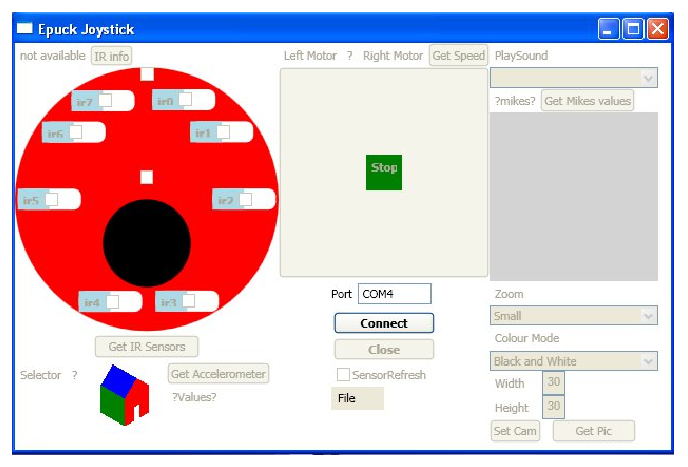
\includegraphics{joystick_start.pdf}}
    \end{picture}%
  \else
    \setlength{\unitlength}{1bp}%
    \begin{picture}(329.22, 223.94)(0,0)
    \put(0,0){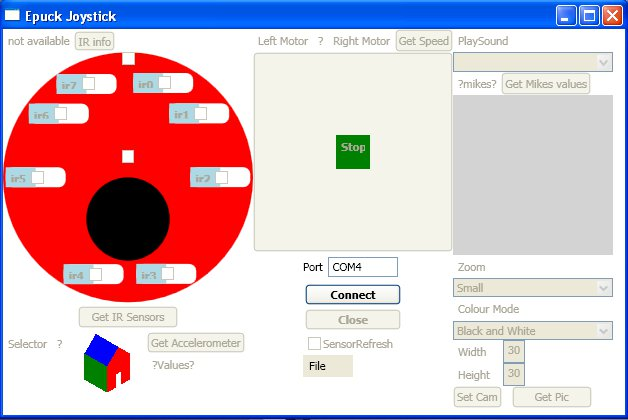
\includegraphics{joystick_start}}
    \end{picture}%
  \fi
  \caption{\label{pic:joystick_start}%
   Elib Joystick start screen}
  \end{figure}


  In the middle there is a connection panel. The connection panel is the only panel, which 
  has activated controls after start up. 
  To activate the rest of controls the following actions are necessary to
  perform. At first pair e-Puck with your computer. Then connect the assigned virtual port with e-Puck.
  Fill the assigned port's name in text box above the "Connect" button and press
  the "Connect" button. After pressing the "Connect" button {\it Elib Joystick} is connected to e-Puck. 
  %todo proc anglicky nejde {\it Elib Joystick} connects to e-Puck?
  The rest of controls are immediately activated
  as soon as the {\it Elib Joystick} is connected to e-Puck.
  See~\ref{sec:copy} guide for detail informations. 
  
  %\input{joystick_log.TpX}
  \begin{figure}[!hbp]
  \centering
  \ifpdf
    \setlength{\unitlength}{1bp}%
    \begin{picture}(326.26, 280.63)(0,0)
    \put(0,0){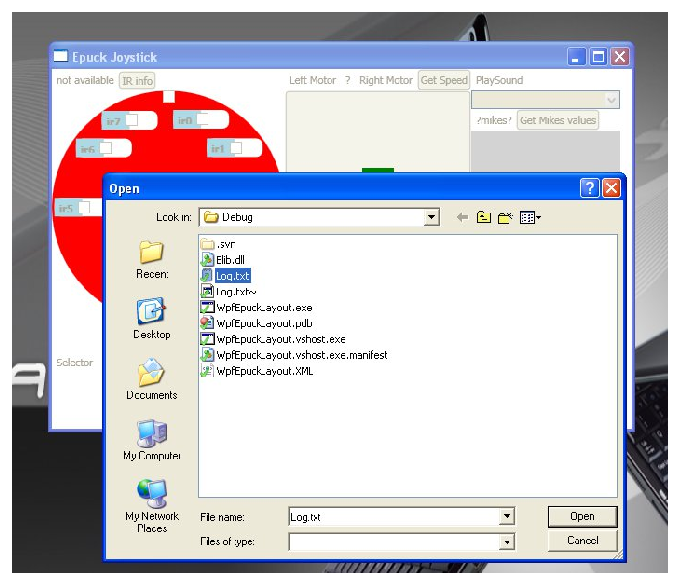
\includegraphics{joystick_log.pdf}}
    \end{picture}%
  \else
    \setlength{\unitlength}{1bp}%
    \begin{picture}(326.26, 280.63)(0,0)
    \put(0,0){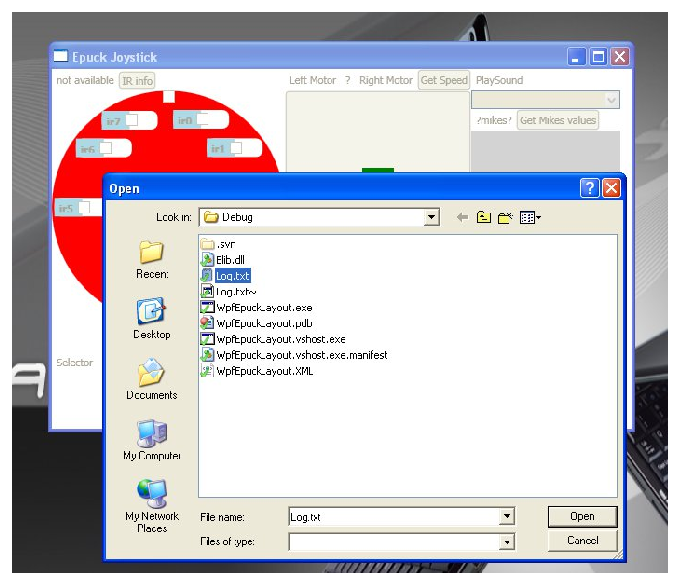
\includegraphics{joystick_log}}
    \end{picture}%
  \fi
  \caption{\label{pic:joystick_log}%
   Optional logging}
  \end{figure}

  The single function available in a non connected state
  is Open File Dialogue depicted on~\ref{pic:joystick_log}.
  In the  Open File Dialogue can be specified the file, 
  where are logged all commands sent to e-Puck after the connection
  to e-Puck is established.

  In order to start using the application connect it to the right serial port and press the "Connect" button.
  Automatically the position of selector is retrieved and the session is established.

  At the beginning all sensors have uninitialised values, 
  which is represented as a question marks in most cases.
  Press the relevant button for retrieving the sensors value. 
  The values will be displayed in the nearest label.
  There are two exceptions. The first exception is the visualization of e-Puck's IR sensors. 
  The values of the IR sensors
  are represented as the blue levels under check boxes on 
  the perimeter of the virtual e-Puck.
  The second  exception is the captured picture, which is displayed enlarged on the right side after its delivery.

  If the connection is too slow or the connection is lost, the application
  is set to initial state. The e-Puck has to be reconnected 
  in order to continue controlling the robot.

  Let us remark that checking the Refresh check box can 
  cause the application to be a little unresponsive.	
  It is so, because the application waits on all values of sensors including an image synchronously.
  On the other hand, a capture and transfer of an image, 
  which was invoked by pressing "Get Pic" button, is performed asynchronously. 
  We have implemented both variants in order to compare the different approaches.

  %\input{joystick_ko.TpX} %lost connection se zachycenym obrazkem a ruznymi hodnotami.
  \begin{figure}[!hbp]
  \centering
  \ifpdf
    \setlength{\unitlength}{1bp}%
    \begin{picture}(293.46, 192.76)(0,0)
    \put(0,0){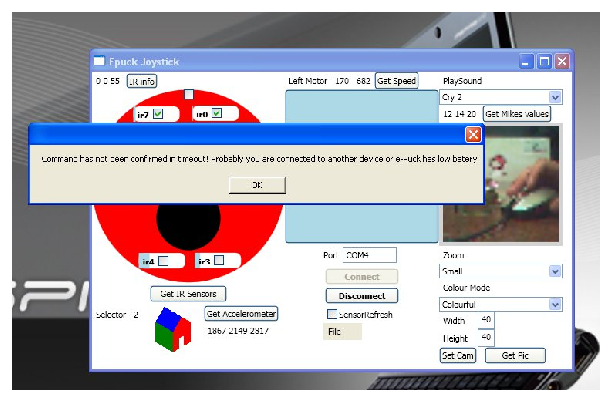
\includegraphics{joystick_ko.pdf}}
    \end{picture}%
  \else
    \setlength{\unitlength}{1bp}%
    \begin{picture}(293.46, 192.76)(0,0)
    \put(0,0){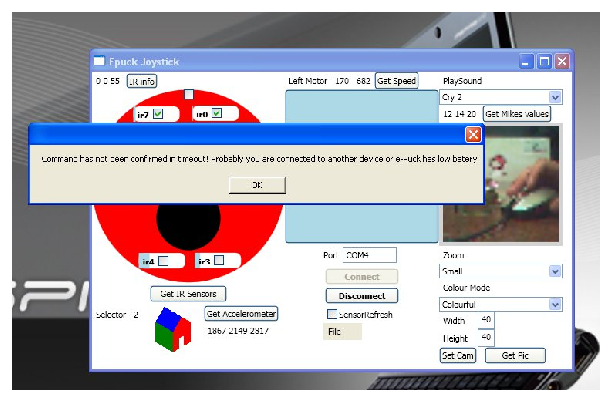
\includegraphics{joystick_ko}}
    \end{picture}%
  \fi
  \caption{\label{pic:joystick_ko}%
   Joystick after Bluetooth connection failure.}
  \end{figure}

  Figure~\ref{pic:joystick_ko} shows the $Message Box$, 
  which tells the user to reconnect the application in order to continue.

  The actuators of e-Puck can be controlled either by clicking 
  on the appropriate button or check box. 
  Another	possibility is to choose a value from combo box.
  The last option is to specify the  convenient values 
  to text boxes and press relevant $set$ button.

  If you want to change the session press the $Disconnect$ button, choose another port and 
  press again "Connect" button or just quit the application and restart it.

  \section{{\it Elib} usage in {\it Elib Joystick}}\label{sec:joystick_trick}
  {\it Elib Joystick} is a graphical application and does not use any sophisticated algorithms. 
  It also uses {\it Elib} really simply in most cases, but there is a crucial problem if the callbacks are used.

  In {\it Elib Joystick} we use callbacks to retrieve an image, because it can last a long time.
  Problems in a graphical application arise if a graphical interface is accessed by a thread different from
  the main thread, where a message loop of the graphical application is running. The problem is solved,
  if all functions use the same thread in the so called Single Thread Apartment (STA).

  {\it Elib Joystick} must solve this problem, because it presents a picture from e-Puck's camera, 
  which is updated in $Label$ of {\it Elib Joystick's} window. 
  The callback, which updates the image, runs in a different thread.
  The problem is solved by using a $Dispatcher$ class. $Dispatcher$ accepts functions, 
  which update the GUI from different threads and calls them in the main thread 
  in order to maintain STA character of GUI. 

\begin{figure}[!hbp]
\begin{lstlisting}
//Ep is instance of e-Puck,
Ep.BeginGetImage(imgto,
  //the callback(lambda function), which is called after an image capture
  (ar) => {
    try {
    Bitmap bmp = Ep.EndGetImage(ar);
    //delegate, which wraps the lambda function that updates the GUI
    updateUIDelegate d = delegate {
      //body of the callback, which updates the GUI
      pic.Source = Convert2BitmapSource(bmp,colorful);
    };
    //updating the GUI by passing the update GUI callback to guid Dispatcher
    guid.Invoke(DispatcherPriority.Normal,d);
    } catch (ElibException) {
      notConfirmedCommand(this);
    }
  }, 
  null
);
\end{lstlisting}
\caption{Update of an image using $Dispatcher$}
\label{updispatcher}
\end{figure}


  The code snippets~\ref{updispatcher} and~\ref{upsynchronous} present usage of the $Dispatcher$ class and 
  synchronous implementation of GUI update. Synchronous update does not require the $Dispatcher$ class,
  because it is performed from main thread.

  The $guid$ $Dispatcher$ used in~\ref{updispatcher} snippet is obtained from the main thread and
  allows the passed functions to access objects as if they were called from the main thread.

\begin{figure}[!hbp]
\begin{lstlisting}
IAsyncResult ar = Ep.BeginGetImage(imgto, null, null);
Bitmap bmp = Ep.EndGetImage(ar);
//pic is a Label
pic.Source = Convert2BitmapSource(bmp,colorful);
\end{lstlisting}
\caption{Synchronous update of an image from the main thread.}
\label{upsynchronous}
\end{figure}
